\documentclass[12pt,a4paper,notitlepage]{report}
\usepackage[utf8]{inputenc}
\usepackage{amsmath}
\usepackage{amsfonts}
\usepackage{amssymb}
\usepackage{graphicx}
\usepackage{listings}

\linespread{1.75}
\title{Lab 1}
\author{Kyle Swanson}

\begin{document}
\maketitle

\begin{normalsize}
	\paragraph*{}
	To begin programming with our new TI Stellaris Launchpads, a logical starting point is the boot loader and the most simple aspects of the system. This lab covered some basic assembly, and using assembly to load information into the different registers. Just as important, we got some experience with the development environment, \emph{IAR Embedded Workbench}. 
	\paragraph*{}
	Since it had been well over a year since I had any exposure to registers, I needed to give myself a quick refresher on how they work and what their purpose is. Put simply, a register is a very small piece of memory, where computer systems usually put their data for doing operations on it. Some registers contain special information, the \emph{Stack Pointer}, \emph{Program Counter}, and \emph{Interrupt Program Status Register} are all examples from this lab. Note figure 1 for examples of different registers. 
	
\begin{figure}[t!]
	\begin{center}
	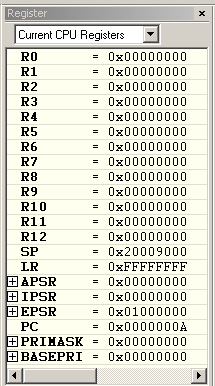
\includegraphics[scale=0.7]{pointers.png}
	\caption{Some of the registers on the TM4C123G}
	\end{center}
\end{figure}	
	
	\paragraph*{}
	These experiments nicely illustrated how registers work. The program we used simply loaded itself, then did an infinite loop. By clicking step by step through the simple program we could watch as it loaded itself into the program counter register, which was one of the most interesting aspects of this lab. When the program loaded, you could watch as the program counter stepped through different addresses, \emph{0x0000000A}, then \emph{0x0000000C}, and so on. This register tells the processor which address to read instructions from. 
	
\pagebreak 
\lstset{language=[x86masm]Assembler}
\begin{lstlisting}
	NAME main
	PUBLIC __iar_program_start
	
	; Interrupt Vector Table
	SECTION .intvec:CODE (2)
	DATA
	DC32 0x20008000U ; Stack Pointer
	DC32 __iar_program_start ; Reset Vector
	
	SECTION LAB1:CODE (2)
	THUMB
	
__iar_program_start
	B main ; Just branch to main
main NOP
	B main ; Loop forever.
	END
		
\end{lstlisting}	
\begin{center}
\small{Figure 2: The infinite loop Assembly source code.}
\end{center}
	
	\paragraph*{}
	At one point, we copied the program from its initial location in memory, and copied it to a different location in memory. Then, you update the program counter register to the new location of the application. This was a difficult task to do, you needed to ensure that the program was allowed access to the portion of memory you were copying it to, and you had to find the program in memory to copy. These problems made me appreciate the complexity of this system. A part that continually confused me across all the experiments was the stack counter. While I learned the absolute basics about the stack pointer in other classes, in practice I found it difficult to relate the assembly commands to their actions, and how it affected the position in memory.
	\paragraph*{} 
	A major aspect of this lab was how computers handle faults, and in the case of this program, how they don't. At its most basic level, a software fault is when a program tries to go outside of its restricted memory. We encountered problems with this while we were trying to copy data between different parts of the program. At times we were completely denied, through the semester, I will have to learn more about memory allocation and how the system gives memory to applications. One register that is closely related to faults is the \emph{IPSR} or \emph{Interrupt Program Status Register}. According to the ARM documentation, this register \emph{"...contains the exception type number of the current Interrupt Service Routine (ISR)."}. Which then relates a interrupt to an fault or other status of the system. This is a register I will need to watch more closely in future labs, it was not until later that I realized the full meaning of this register. The following is a few of the status codes that may be loaded into the \emph{IPSR}.
\begin{itemize}
  \item 1 = Reserved
  \item 2 = NMI
  \item 3 = HardFault
\end{itemize}
From what I read, a system should not crash during a fault, it should switch the program counter to a non-faulted portion, and continue running. 

\paragraph*{}
I found that generally, when instructions were set away from the defaults that the system pushes you towards, you got strange and unexpected results. For instance, when we placed executable instructions where it expected to find the \emph{Stack Pointer}, it first complained that the \emph{\_\_vector\_table symbol not found}. It then stated that the \emph{Stack addr = 0x00000009}, this implies to me that the \emph{\_\_iar\_program\_start} really just equals 0x00000009. Which I assume is the location the system starts at. This portion was cut short, since the system seemed to crash in this configuration. All the registers displayed as empty, the memory said it was blank, but as far as I can tell, the system was running. 

\paragraph*{}
These experiments were a good way to get a very basic understanding of ARM processors and the TI platform and work environment. Having more questions in my head than when I started will help me watch and learn in more specific ways in future labs, than simply being lost. Which happened a few times in this initial lab. This was a good refresher into computer architecture, since it has been so long since my last exposure to registers, hex, and assembly has been over a year. 

\end{normalsize}

\end{document}